\documentclass[border=10pt]{standalone}
\usepackage{tikz}
\usetikzlibrary{arrows.meta, shapes, calc}

\begin{document}

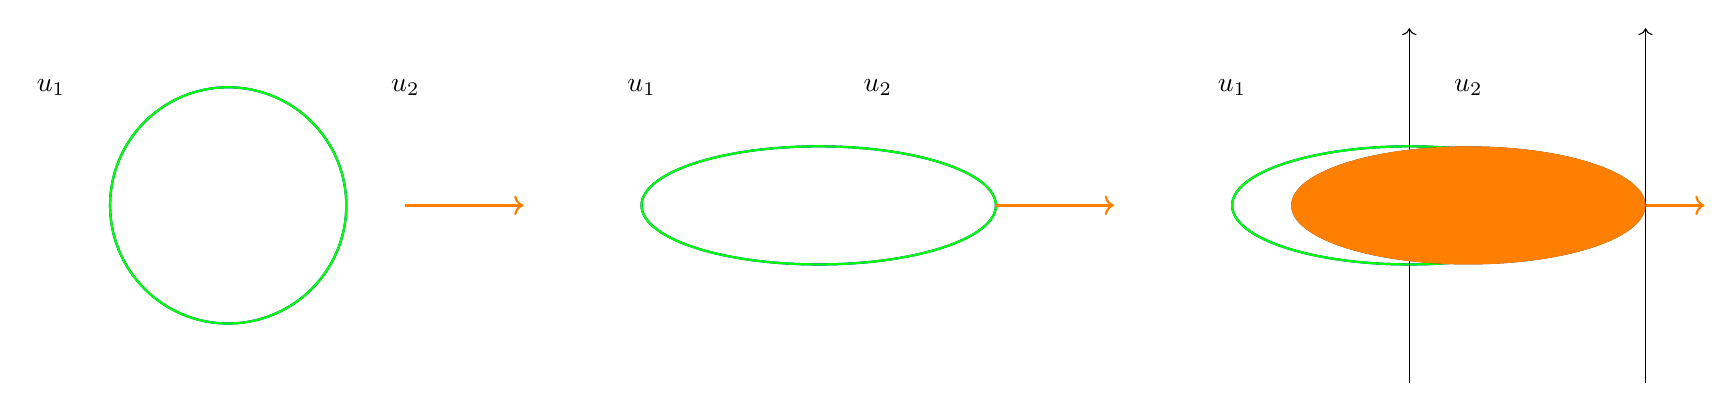
\begin{tikzpicture}[scale=1.5]
    % First subplot
    \draw[thick, blue] (0,0) circle (1);
    \draw[thick, green] (0,0) circle (1);
    \draw[thick, orange, ->] (1.5,0) -- (2.5,0);
    \node at (-1.5,1) {$u_1$};
    \node at (1.5,1) {$u_2$};
    
    % Second subplot
    \draw[thick, blue] (5,0) ellipse (1.5 and 0.5);
    \draw[thick, green] (5,0) ellipse (1.5 and 0.5);
    \draw[thick, orange, ->] (6.5,0) -- (7.5,0);
    \node at (3.5,1) {$u_1$};
    \node at (5.5,1) {$u_2$};
    
    % Third subplot
    \draw[thick, blue] (10,0) ellipse (1.5 and 0.5);
    \draw[thick, green] (10,0) ellipse (1.5 and 0.5);
    \draw[thick, orange, ->] (11.5,0) -- (12.5,0);
    \node at (8.5,1) {$u_1$};
    \node at (10.5,1) {$u_2$};
    
    % Axes for the third subplot
    \draw[->] (10,-1.5) -- (10,1.5);
    \draw[->] (12,-1.5) -- (12,1.5);
    
    % Fill the intersection area
    \fill[black!80] (10.5,0) ellipse (1.5 and 0.5);
    \fill[orange] (10.5,0) ellipse (1.5 and 0.5);
\end{tikzpicture}

\end{document}